\documentclass[a4paper,10pt]{article}
\usepackage[brazil]{babel}
\usepackage[utf8]{inputenc}
\usepackage[T1]{fontenc}
\usepackage{psfrag}
\usepackage{times}
\usepackage{indentfirst}
\usepackage{amsmath,amsfonts,amssymb}
\usepackage{graphicx}
\usepackage{mathtools}
\usepackage{url}

\urlstyle{tt}
\emergencystretch=3em


\title{\textbf{Programação em Tempo Real para Sistemas Embarcados} \\ \vspace{1.0cm} \textbf{Relatório Projeto Final - Módulo de Interface via Display} \\  \vspace{1.0cm} \large Professor: Jes de Jesus Fiais Cerqueira \\ \vspace{2.5cm}

\includegraphics[width=4.5cm]{brasao_ufba.jpg} \vspace{1.0cm} }

\author{David Ferrari, João Cerqueira, Vinícius Jesus, Felipe Cunha \\
Universidade Federal da Bahia, Campus Salvador}
\date{Julho, 2026}

\begin{document}
\maketitle

\clearpage

\renewcommand*\contentsname{Sumário}

\tableofcontents

\clearpage



\section{Introdução}

Sistemas embarcados aplicados à robótica móvel exigem a integração de diferentes funções, como aquisição de dados, processamento, comunicação, controle e interface com o usuário. Em uma base robótica móvel, como em arquiteturas com várias rodas e diferentes sensores coletando dados, diversas grandezas precisam ser acompanhadas continuamente para que o estado do sistema possa ser devidamente supervisionado. Entre essas grandezas estão as correntes dos motores, as velocidades angulares das rodas, as velocidades lineares da base e as informações de posição.

No contexto da disciplina \textit{Programação em Tempo Real para Sistemas Embarcados}, o projeto final foi organizado como parte de uma solução maior voltada ao controle e monitoramento de uma base robótica móvel. Cada equipe ficou responsável por um módulo específico do sistema, permitindo que o problema fosse dividido em partes menores e mais bem definidas. Neste trabalho, estudar-se-á o desenvolvimento do módulo de interface via display, cuja função é apresentar, de forma organizada, informações relevantes de telemetria do robô em estudo.

O módulo desenvolvido utiliza a placa Black Pill, baseada no microcontrolador STM32F411CEU6, em conjunto com um display OLED SSD1306 monocromático de resolução $128 \times 64$ pixels. A comunicação entre o microcontrolador e o display é realizada por meio do barramento I2C, escolha coerente com a proposta do projeto e paralela à aplicações embarcadas presentes no mercado.

A implementação foi construída sobre o FreeRTOS, sistema operacional de tempo real utilizado para estruturar a aplicação em tarefas concorrentes e muito presente no mercado. Essa escolha permite representar, de maneira mais próxima de um sistema real, a existência de diferentes fluxos de dados operando com períodos distintos. No projeto, dados de corrente, velocidade angular e posição são simulados por tabelas de valores e processados por tarefas periódicas. A comunicação entre as tarefas é realizada por filas do FreeRTOS, enquanto o acesso às variáveis globais compartilhadas é protegido por mutexes. Dessa forma, o firmware separa a geração dos dados, a leitura das filas, o processamento das grandezas e a atualização da interface gráfica.

Além da simples exibição de valores no display, o módulo também realiza a transformação das velocidades angulares das três rodas em grandezas associadas ao movimento da base robótica, como as velocidades lineares nos eixos $x$ e $y$ e a velocidade angular do corpo do robô. Essas informações são organizadas em três telas principais: uma tela para velocidade linear e posição, uma tela para velocidades angulares das rodas e velocidade angular do robô, e uma tela para as correntes dos motores. A alternância entre essas telas é feita por meio de um botão conectado ao pino PA0, tratado por interrupção externa, com notificação da tarefa responsável pelo gerenciamento do display.

Como nem todos os sensores e módulos físicos do sistema completo estavam disponíveis para integração, a validação do firmware foi realizada por meio de simulações. O ambiente Renode foi utilizado para executar o firmware compilado para o STM32, observar mensagens de depuração via UART, testar a troca de telas por botão virtual, verificar a comunicação I2C com o dispositivo OLED simulado e capturar o conteúdo real do framebuffer do driver SSD1306. Essa abordagem permitiu validar não apenas a lógica funcional da interface, mas também aspectos importantes de sistemas de tempo real, como periodicidade de tarefas, comunicação entre tarefas, exclusão mútua, interrupções e atualização de periféricos.

A Figura~\ref{fig:modulo} apresenta o módulo de interface dentro da proposta geral do projeto.

\begin{figure}[h]
    \centering
    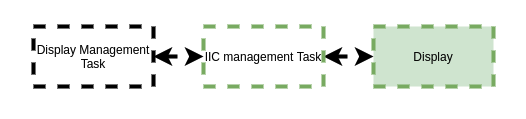
\includegraphics[width=0.7\linewidth]{modulo.png}
    \caption{Módulo de interface via display desenvolvido no projeto.}
    \label{fig:modulo}
\end{figure}

\section{Objetivos}

O objetivo geral deste trabalho é desenvolver e validar um módulo de interface com um  display para uma base robótica móvel, utilizando um sistema embarcado baseado no microcontrolador STM32F411CEU6, no sistema operacional de tempo real FreeRTOS e em um display OLED SSD1306 com comunicação I2C.

O módulo tem como finalidade organizar e exibir informações relevantes de telemetria do robô, tais como correntes dos motores, velocidades angulares das rodas, velocidades lineares estimadas e posição. Como os sensores físicos e os demais módulos do sistema completo não estavam integrados ao ambiente de desenvolvimento, os dados de entrada foram simulados por meio de tabelas de valores (lookup table), permitindo validar a lógica de aquisição, processamento, comunicação entre tarefas e atualização da interface gráfica.

De forma mais específica, este trabalho tem como objetivos:

\begin{itemize}
    \item modelar os dados de corrente, velocidade angular e posição em uma estrutura comum, adequada ao uso em filas do FreeRTOS;

    \item simular a geração de dados de sensores por meio de tabelas de valores armazenadas em memória;

    \item implementar tarefas periódicas responsáveis pela geração dos dados simulados em diferentes taxas de atualização;

    \item utilizar filas do FreeRTOS para desacoplar a produção e o consumo dos dados;

    \item implementar tarefas leitoras responsáveis por consumir as filas e atualizar o estado mais recente do sistema;

    \item proteger o acesso às variáveis globais compartilhadas por meio de mutexes, evitando condições de corrida entre as tarefas leitoras e a tarefa de display;

    \item calcular as velocidades lineares da base robótica a partir das velocidades angulares das três rodas, considerando a cinemática de uma base omnidirecional;

    \item desenvolver três telas de exibição no display OLED SSD1306: uma para velocidade linear e posição, uma para velocidades angulares e uma para correntes dos motores;

    \item implementar a troca de telas por meio de botão conectado ao pino PA0, utilizando interrupção externa e notificação de tarefa no FreeRTOS;

    \item utilizar a UART2 como recurso auxiliar de \textbf{depuração} e simulação no ambiente Renode;

    \item validar o funcionamento do firmware por meio de simulações, verificando a criação das tarefas, a comunicação por filas, a troca de telas, a comunicação I2C com o OLED e a geração do conteúdo gráfico no framebuffer do driver SSD1306.
\end{itemize}

Assim, o foco do projeto não está no controle completo da base robótica, mas na implementação de um módulo de interface embarcado, capaz de receber ou simular informações do sistema, processar de maneira concorrente e apresentar de forma organizada em um oled.

\section{Desenvolvimento}

\subsection{Solução adotada}

Para solucionar o problema, primeiramente definimos como organizaríamos os dados a serem mostrados, afinal em sistemas embarcados os recursos são escassos e uma boa modelagem garante performance, segurança e escalabilidade do projeto, sendo parte fundamental do processo.

Como precisamos mostrar:
\begin{itemize}
    \item Posição ($x$, $y$);
    \item Velocidade angular das rodas (entrada dos sensores);
    \item Velocidade linear e velocidade angular do robô (grandezas derivadas);
    \item Corrente em cada motor.
\end{itemize}

Escolhemos propositalmente construir uma struct de três dimensões, $x$, $y$ e $z$, e um campo \texttt{TickType\_t timestamp} como segue:

\begin{verbatim}
    typedef struct {
        float x;
        float y;
        float z;
        TickType_t timestamp;
    } dataset;
\end{verbatim}

Dessa forma temos de ganho:
\begin{itemize}
    \item Uma só definição de fila, todas as filas usam \texttt{sizeof(dataset)} como tamanho de elemento, e as tarefas leitoras/produtoras compartilham a mesma lógica;
    \item Menos código duplicado, as funções de tela, os mutexes e o padrão produtor/consumidor funcionam igual para qualquer grandeza;
    \item Timestamp comum, toda amostra carrega o tick de geração, útil para rastrear latência/ordem.
\end{itemize}

Como o robô tem 3 rodas, temos 3 valores de corrente e 3 valores de velocidade angular, que ocupam integralmente os campos $x$, $y$ e $z$. Já a posição usa apenas $x$ e $y$, ficando o campo $z$ sem uso nesse caso. O reaproveitamento acontece no dataset de velocidade linear, grandeza derivada da transformação: os campos $x$ e $y$ guardam $V_x$ e $V_y$, e o campo $z$ guarda a velocidade angular do corpo do robô ($\omega$), calculada na mesma etapa. Dessa forma nada é perdido e conseguimos representar todo o estado do robô para então ser enviado ao display.

Definida a modelagem dos dados, a arquitetura do sistema segue o padrão produtor/consumidor sobre as filas do FreeRTOS. Para cada grandeza existe uma tarefa produtora, que gera as amostras na taxa do respectivo sensor e as deposita em uma fila dedicada, e uma tarefa consumidora, que drena essa fila, aplica as transformações necessárias e publica o valor mais recente em uma variável global protegida por mutex, de onde a tarefa de display faz a leitura. Esse desacoplamento permite que cada lado opere em seu próprio ritmo, os produtores rodam com prioridades altas e períodos curtos, enquanto os consumidores e a interface rodam mais lentamente, sem que um bloqueie o outro. As filas absorvem rajadas de produção e, por serem estruturas thread-safe do próprio RTOS, dispensam sincronização manual no hand-off entre tarefas, a exclusão mútua explícita fica restrita ao ponto em que consumidores e display compartilham o estado final do robô.

\subsection{Geração dos dados}

Como o projeto não dispõe dos sensores físicos, os dados de entrada são simulados por meio de tabelas de consulta (lookup tables). Um script em Python (\texttt{generate-lookup-table.py}) gera, em tempo de compilação, nove vetores de 100 posições com valores aleatórios dentro de faixas realistas para cada grandeza: corrente de 0 a 4 A, velocidade angular de 0 a $10\pi$ rad/s e posição de 0 a 1000 cm. O resultado é escrito diretamente no arquivo \texttt{lookuptable.c}, que é compilado junto ao firmware, evitando qualquer custo de geração em tempo de execução.

Dentro do sistema embarcado, três tarefas produtoras percorrem esses vetores de forma circular, simulando um fluxo contínuo de amostras. Cada tarefa monta um \texttt{dataset} com os três valores da sua grandeza e o tick atual do RTOS como timestamp, e o envia para a fila correspondente com \texttt{xQueueSendToBack} sem bloqueio. Os períodos foram definidos para refletir a dinâmica de cada sensor: corrente a cada 1 ms (fila de 50 elementos), velocidade angular a cada 10 ms (fila de 30) e posição a cada 100 ms (fila de 5). A periodicidade é garantida por \texttt{vTaskDelayUntil}, que mantém o período fixo sem acúmulo de atraso. Caso alguma fila encha, o dado é descartado e o LED da placa sinaliza a condição de overflow.

\subsection{Transformação dos dados}

A transformação principal ocorre na tarefa leitora de velocidade angular. As lookup tables fornecem as velocidades angulares das três rodas ($M_1$, $M_2$, $M_3$), mas a interface deve exibir a velocidade do robô como corpo. Para isso aplica-se a cinemática direta de uma base omnidirecional de três rodas dispostas a $120^{\circ}$ (ângulos $\alpha$ de $0^{\circ}$, $120^{\circ}$ e $240^{\circ}$), com raio de roda $r = 5$ cm e distância do centro à roda $L = 10$ cm:

\begin{align*}
V_x &= r \cdot \frac{2}{3} \cdot \left[ -\operatorname{sen}(\alpha_1) M_1 - \operatorname{sen}(\alpha_2) M_2 - \operatorname{sen}(\alpha_3) M_3 \right] \\
V_y &= r \cdot \frac{2}{3} \cdot \left[ \cos(\alpha_1) M_1 + \cos(\alpha_2) M_2 + \cos(\alpha_3) M_3 \right] \\
\omega &= \frac{r \left( M_1 + M_2 + M_3 \right)}{3L}
\end{align*}

Os senos e os cossenos são pré-calculados como constantes na inicialização da tarefa, evitando chamadas trigonométricas repetidas a cada amostra. O resultado é armazenado em um \texttt{dataset} de velocidade linear, com $V_x$ e $V_y$ nos campos $x$ e $y$, e a velocidade angular do corpo $\omega$ reaproveitando o campo $z$. Cada tarefa leitora esvazia sua fila em laço e grava o valor mais recente na variável global de snapshot correspondente, sempre protegida por mutex (padrão take, escreve, give, com timeout de 1 ms), garantindo exclusão mútua com a tarefa de exibição.

\subsection{Envio ao display}

A comunicação com o display OLED SSD1306 é feita pelo barramento I2C1 a 400 kHz (pinos PB6/SCL e PB7/SDA), com o display no endereço \texttt{0x3C}. O driver mantém um framebuffer de 1 KB em RAM ($128 \times 64$ pixels, 1 bit por pixel); as funções de desenho de texto e primitivas escrevem apenas nesse buffer, e a função \texttt{SSD1306\_UpdateScreen} transfere o buffer completo ao display via HAL. Isso reduz o número de transações I2C e evita cintilação.

A tarefa \texttt{vDisplayManager}, de menor prioridade do sistema, gerencia três telas: velocidade linear e posição, velocidade angular, e correntes dos motores. Ela bloqueia em \texttt{ulTaskNotifyTake} com timeout de 699 ms. Se o timeout expira, apenas os valores da tela atual são atualizados, lendo as variáveis globais sob mutex. Se uma notificação chega, a tela avança ciclicamente e é redesenhada por completo.

A notificação vem do botão KEY (PA0), tratado por interrupção externa. O pressionamento gera uma borda de descida que dispara a EXTI0; o handler \texttt{EXTI0\_IRQHandler} delega ao HAL, que invoca o callback \texttt{HAL\_GPIO\_EXTI\_Callback} reimplementado na aplicação. Nele aplica-se um debounce por software de 200 ms, necessário porque o botão da placa não possui filtro de hardware, e em seguida a tarefa de display é acordada com \texttt{vTaskNotifyGiveFromISR}, seguida de \texttt{portYIELD\_FROM\_ISR} para troca de contexto imediata. Esse é o padrão de interrupção diferida: a ISR faz o mínimo e o trabalho pesado fica em contexto de tarefa. A EXTI0 foi configurada com prioridade 5, o valor mais urgente permitido pelo \texttt{configMAX\_SYSCALL\_INTERRUPT\_PRIORITY} do FreeRTOS para ISRs que chamam APIs \texttt{FromISR}.

Além da EXTI0, o sistema usa as interrupções de infraestrutura do RTOS: o SysTick gera o tick do escalonador, o par PendSV/SVC realiza as trocas de contexto e o TIM1 serve como base de tempo do HAL, já que o SysTick fica dedicado ao FreeRTOS. Quanto aos handlers de objetos do RTOS, o sistema mantém três \texttt{QueueHandle\_t} (uma fila por grandeza), quatro \texttt{SemaphoreHandle\_t} (um mutex por variável global compartilhada) e um \texttt{TaskHandle\_t} da tarefa de display, usado como alvo da notificação enviada pela interrupção do botão.

\subsection{Pinagem}

Utilizando os equipamentos citados anteriormente, a pinagem do projeto ficou como segue na imagem.

\begin{figure}[h]
    \centering
    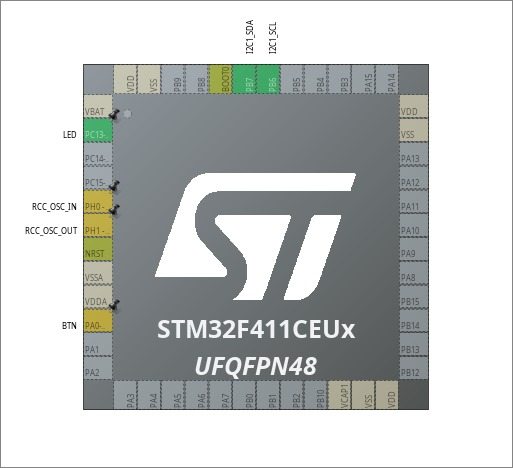
\includegraphics[width=0.7\linewidth]{pinagem.jpeg}
    \caption{Planejamento dos pinos para o STM32F411CEUx}
    \label{fig:pinagem}
\end{figure}

\begin{itemize}
    \item \textbf{LED (PC13):} Alimenta o LED indicador da placa. No firmware, é apagado quando ocorre overflow em alguma das filas FreeRTOS.
    \item \textbf{BTN (PA0):} Botão KEY da Black Pill. Dispara a interrupção EXTI0 (borda de descida, pull-up interno) para trocar a tela exibida no OLED.
    \item \textbf{I2C1\_SCL (PB6):} Pino de clock da interface I2C1, essencial para a comunicação com o display OLED SSD1306.
    \item \textbf{I2C1\_SDA (PB7):} Pino de dados da interface I2C1, essencial para a comunicação com o display OLED SSD1306.
    \item \textbf{RCC\_OSC\_IN / RCC\_OSC\_OUT (PH0 / PH1):} Pinos do oscilador externo (cristal).
\end{itemize}

\section{Simulações e Validação}

A validação do módulo de interface foi realizada com o \textit{Renode}, utilizado para executar o firmware compilado para o microcontrolador STM32F411CEU6 em um ambiente simulado. Essa etapa foi importante porque permitiu verificar o comportamento do sistema mesmo sem a integração completa com todos os sensores e periféricos físicos da base robótica.

As simulações tiveram como objetivo validar o fluxo principal do firmware, desde a geração dos dados simulados até a atualização da interface gráfica. De forma geral, o caminho verificado foi:

\begin{verbatim}
lookuptable.c
-> tasks geradoras FreeRTOS
-> filas
-> tasks leitoras
-> mutexes
-> variáveis globais
-> gerenciador de display
-> driver SSD1306
-> I2C1
-> OLED simulado no endereço 0x3C
\end{verbatim}

Além disso, a UART2 foi utilizada como recurso auxiliar de depuração. É importante destacar que a UART2 não substitui o display OLED no projeto. Ela foi usada apenas para observar, no terminal, o comportamento interno do firmware durante a simulação, permitindo acompanhar a criação das tarefas, os valores exibidos nas telas, os comandos de troca de tela e os resultados dos testes. Isso foi extremamente importante, principalmente pela ausência de simuladores específicos para esse trabalho, como a falta do OLED.

\subsection{Uso da UART2 como recurso de depuração}

A primeira etapa de validação consistiu em utilizar a UART2 para observar a execução do firmware no Renode. A UART foi conectada a uma porta TCP, permitindo a visualização das mensagens de debug por meio de um terminal no computador. O firmware foi iniciado no Renode com o script de simulação e, em outro terminal, a saída serial foi acompanhada com o comando:

\begin{verbatim}
nc localhost 12345
\end{verbatim}

Na inicialização, a UART permitiu confirmar a criação das principais tarefas do FreeRTOS. Foram observadas mensagens indicando a criação da task gerenciadora do display, das tasks produtoras de dados, das tasks leitoras de filas e da task auxiliar de comandos de simulação:

\begin{verbatim}
INIT RTOS | heap before tasks=30784
CREATE displayManager=1
CREATE gerarQueueCorrente=1
CREATE gerarQueueVelAngular=1
CREATE gerarQueuePosicao=1
CREATE queueCorrenteReader=1
CREATE queueVelAngularReader=1
CREATE queuePosicaoReader=1
CREATE simCommandReader=1
\end{verbatim}

Esse resultado confirmou que o FreeRTOS foi iniciado corretamente e que o heap disponível foi suficiente para criar os objetos principais da aplicação. Também foi possível observar, pela UART, os valores que estavam sendo enviados para cada uma das telas do display.

Na \texttt{SCREEN1}, por exemplo, foram exibidas as velocidades lineares calculadas e os valores de posição:

\begin{verbatim}
SCREEN1 | Vx=24.0 | Vy=-142.2 | Px=472.67 | Py=737.60
SCREEN1 | Vx=-215.9 | Vy=145.5 | Px=942.74 | Py=125.76
\end{verbatim}

Essas mensagens permitiram verificar que os dados estavam sendo gerados, processados pelas tasks leitoras, armazenados nas variáveis globais protegidas por mutexes e finalmente acessados pela task de display.

\subsection{Teste de troca de telas via UART}

Após confirmar a execução básica do firmware, foi realizado um teste de troca de telas por meio da UART2. Para isso, a task auxiliar \texttt{vTaskSimCommandReader} foi utilizada para receber comandos de simulação. Ao digitar o caractere \texttt{n}, o firmware enviava uma notificação à task \texttt{vDisplayManager}, solicitando a troca para a próxima tela.

A sequência esperada era:

\begin{verbatim}
SCREEN1 -> SCREEN2 -> SCREEN3 -> SCREEN1
\end{verbatim}

Durante o teste, a aplicação iniciou na \texttt{SCREEN1}. Após o envio do comando \texttt{n}, a tela mudou para a \texttt{SCREEN2}, responsável por apresentar as velocidades angulares das três rodas e a velocidade angular do corpo do robô. Um novo envio do comando levou à \texttt{SCREEN3}, que apresenta as correntes dos motores. Ao enviar o comando novamente, o sistema retornou para a \texttt{SCREEN1}.

Esse teste confirmou que a lógica de alternância entre telas funcionava corretamente e que a task gerenciadora do display respondia às notificações recebidas. No entanto, esse mecanismo foi utilizado apenas como ferramenta de simulação e depuração. No funcionamento previsto para o módulo, a troca de telas é realizada pelo botão conectado ao pino PA0.

\begin{figure}
    \centering
    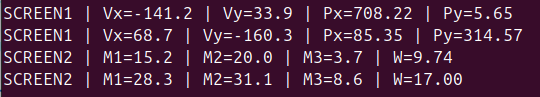
\includegraphics[width=0.5\linewidth]{mudança.png}
    \caption{Mudança nos screens}
    \label{fig:placeholder}
\end{figure}

\subsection{Teste do botão virtual PA0 e interrupção EXTI0}

Depois da validação da troca de telas via UART, foi realizado um teste mais próximo do comportamento esperado no hardware físico. O botão foi configurado no pino PA0, utilizando interrupção externa pela linha EXTI0. No Renode, o botão virtual foi acionado por meio dos comandos:

\begin{verbatim}
sysbus.gpioPortA.UserButton Press
sysbus.gpioPortA.UserButton Release
\end{verbatim}

O fluxo esperado para esse teste era:

\begin{verbatim}
botão virtual
-> GPIOA/PA0
-> EXTI0
-> EXTI0_IRQHandler()
-> HAL_GPIO_EXTI_IRQHandler(GPIO_PIN_0)
-> HAL_GPIO_EXTI_Callback(GPIO_PIN_0)
-> vTaskNotifyGiveFromISR()
-> vDisplayManager
-> troca de tela
\end{verbatim}

A interrupção foi tratada no arquivo \texttt{stm32f4xx\_it.c}, por meio da função:

\begin{verbatim}
void EXTI0_IRQHandler(void)
{
    HAL_GPIO_EXTI_IRQHandler(GPIO_PIN_0);
}
\end{verbatim}

No callback \texttt{HAL\_GPIO\_EXTI\_Callback}, foi implementado um debounce por software de 200 ms, evitando que ruídos ou múltiplas transições rápidas do botão gerassem várias trocas de tela indevidas. A interrupção não executa diretamente a atualização da tela; ela apenas notifica a task de display por meio da função \texttt{vTaskNotifyGiveFromISR}. Essa abordagem é adequada para sistemas de tempo real, pois mantém a rotina de interrupção curta e transfere o processamento da interface para o contexto da task.

O teste confirmou que o botão virtual do Renode acionou corretamente a interrupção EXTI0 e que a task \texttt{vDisplayManager} realizou a troca de tela. Assim, foi validado o mecanismo real previsto para a interação do usuário com o módulo.

\subsection{Teste de comunicação I2C com o OLED SSD1306}

No ambiente Renode, o OLED foi representado por um dispositivo I2C simulado no endereço \texttt{0x3C}, o mesmo endereço utilizado pelo driver SSD1306 no firmware. Para verificar se as chamadas de atualização do display estavam de fato chegando ao barramento I2C, foram adicionados contadores no driver:

\begin{verbatim}
ssd1306_i2c_ok_count
ssd1306_i2c_err_count
\end{verbatim}

Esses contadores registram, respectivamente, transmissões I2C bem-sucedidas e transmissões com erro. Durante o teste, os contadores foram lidos diretamente da memória simulada do microcontrolador. O resultado observado foi:

\begin{verbatim}
ssd1306_i2c_ok_count  = 0x00010701
ssd1306_i2c_err_count = 0x00000000
\end{verbatim}

Convertendo o primeiro valor para decimal:

\[
0x00010701 = 67329
\]

Portanto, durante a simulação, foram registradas 67329 escritas I2C bem-sucedidas e nenhum erro de comunicação. Esse resultado indicou que o firmware estava executando o caminho real de atualização do display, passando pelo driver SSD1306, pela HAL I2C, pelo barramento I2C1 e pelo dispositivo OLED simulado no Renode.

\subsection{Captura e renderização do framebuffer do OLED}

Uma limitação da configuração utilizada no Renode é que o OLED SSD1306 não é renderizado automaticamente como uma tela gráfica de $128 \times 64$ pixels. O periférico simulado permite validar a comunicação no barramento I2C, mas não mostra visualmente os pixels enviados para o display.

Para contornar essa limitação, foi adotada uma estratégia complementar: capturar diretamente o framebuffer do driver SSD1306 na memória simulada. O display possui resolução de $128 \times 64$ pixels e é monocromático. Como cada pixel é representado por 1 bit, o tamanho total do framebuffer é:

\[
128 \times 64 \div 8 = 1024 \text{ bytes}
\]

No driver, o framebuffer é declarado como:

\begin{verbatim}
static uint8_t ssd1306_buffer[SSD1306_BUFFER_SIZE];
\end{verbatim}

Após localizar o endereço desse buffer no arquivo ELF gerado pela compilação, foi criado um script para ler os 1024 bytes correspondentes diretamente da memória simulada. Em seguida, outro script em Python interpretou esse conteúdo no formato utilizado pelo SSD1306, em que cada byte representa 8 pixels verticais, e gerou imagens PNG das telas.

Essa etapa foi importante porque as imagens geradas não vieram da UART, mas sim do conteúdo real do framebuffer preparado pelo driver SSD1306. Portanto, a validação visual confirmou que o firmware estava desenhando corretamente as telas que seriam enviadas ao OLED físico.

A Figura~\ref{fig:screen1_sim} apresenta uma captura da \texttt{SCREEN1}, contendo velocidade linear e posição.

\begin{figure}[h]
    \centering
    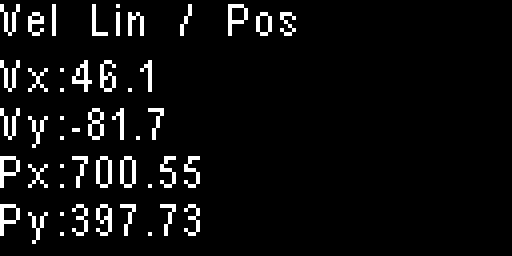
\includegraphics[width=0.65\linewidth]{screen1.png}
    \caption{Captura renderizada do framebuffer da \texttt{SCREEN1}, exibindo velocidade linear e posição.}
    \label{fig:screen1_sim}
\end{figure}

A Figura~\ref{fig:screen2_sim} apresenta uma captura da \texttt{SCREEN2}, contendo as velocidades angulares das rodas e a velocidade angular do robô.

\begin{figure}[h]
    \centering
    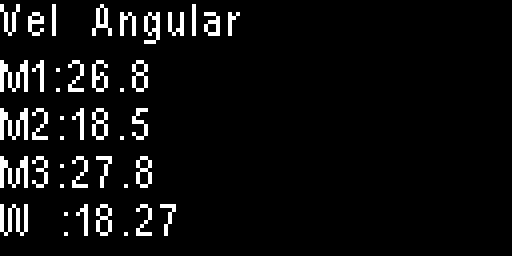
\includegraphics[width=0.65\linewidth]{screen2.png}
    \caption{Captura renderizada do framebuffer da \texttt{SCREEN2}, exibindo velocidades angulares.}
    \label{fig:screen2_sim}
\end{figure}

\begin{figure}[h]
    \centering
    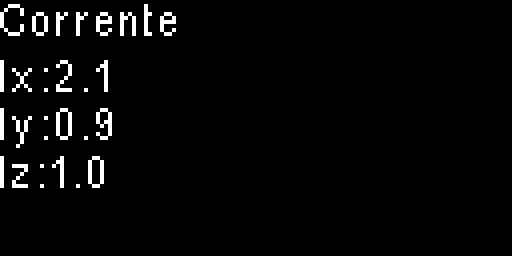
\includegraphics[width=0.65\linewidth]{screen3.png}
    \caption{Captura renderizada do framebuffer da \texttt{SCREEN3}, exibindo correntes.}
    \label{fig:screen2_sim}
\end{figure}

\subsection{Teste de temporização das tasks}

Além dos testes funcionais, foi realizada uma simulação específica para verificar a temporização das tasks do FreeRTOS. Para isso, foram adicionados contadores globais ao firmware, incrementados a cada execução das tasks geradoras, leitoras e da task de display. Também foi criada uma task auxiliar, chamada \texttt{vTaskTimingMonitor}, responsável por imprimir, a cada 10 segundos, a quantidade de execuções observada em cada task.

A janela de observação utilizada foi definida por:

\begin{verbatim}
#define TIMING_MONITOR_WINDOW_MS 10000
\end{verbatim}

Os períodos configurados no firmware são apresentados na Tabela~\ref{tab:periodos_tasks}.

\begin{table}[h]
\centering
\renewcommand{\arraystretch}{1.3}
\begin{tabular}{|p{5.2cm}|p{3.2cm}|p{4.2cm}|}
\hline
\textbf{Task} & \textbf{Período} & \textbf{Execuções esperadas em 10 s} \\
\hline
Geração de corrente & 1 ms & 10000 \\
\hline
Geração de velocidade angular & 10 ms & 1000 \\
\hline
Geração de posição & 100 ms & 100 \\
\hline
Leitura da fila de corrente & 25 ms & 400 \\
\hline
Leitura da fila de velocidade angular & 100 ms & 100 \\
\hline
Leitura da fila de posição & 125 ms & 80 \\
\hline
Atualização do display & 700 ms & aproximadamente 14 ativações nominais \\
\hline
\end{tabular}
\caption{Períodos configurados para as principais tasks do firmware.}
\label{tab:periodos_tasks}
\end{table}

Durante a simulação, foram observadas duas janelas consecutivas de 10 segundos. Os resultados obtidos foram:

\begin{verbatim}
TASK TIMING | janela=10000 ms
GEN  | corrente=10006 | velAngular=1001 | posicao=100
READ | corrente=400 | velAngular=100 | posicao=81
DISP | display=5

TASK TIMING | janela=10000 ms
GEN  | corrente=10005 | velAngular=1001 | posicao=100
READ | corrente=401 | velAngular=100 | posicao=80
DISP | display=4
\end{verbatim}

A Tabela~\ref{tab:resultado_temporizacao} compara os valores esperados com os valores observados.

\begin{table}[h]
\centering
\renewcommand{\arraystretch}{1.3}
\begin{tabular}{|p{5.2cm}|p{3.2cm}|p{4.2cm}|}
\hline
\textbf{Task} & \textbf{Esperado em 10 s} & \textbf{Observado} \\
\hline
Geração de corrente & 10000 & 10005--10006 \\
\hline
Geração de velocidade angular & 1000 & 1001 \\
\hline
Geração de posição & 100 & 100 \\
\hline
Leitura da fila de corrente & 400 & 400--401 \\
\hline
Leitura da fila de velocidade angular & 100 & 100 \\
\hline
Leitura da fila de posição & 80 & 80--81 \\
\hline
Atualização completa do display & aproximadamente 14 ativações nominais & 4--5 atualizações completas \\
\hline
\end{tabular}
\caption{Resultado observado no teste de temporização das tasks.}
\label{tab:resultado_temporizacao}
\end{table}

Os resultados mostram que as tasks geradoras e leitoras apresentaram contagens compatíveis com os períodos definidos no firmware. A geração de corrente, configurada para ocorrer a cada 1 ms, executou cerca de 10000 vezes em 10 segundos. A geração de velocidade angular, com período de 10 ms, executou cerca de 1000 vezes. A geração de posição, com período de 100 ms, executou exatamente 100 vezes nas janelas observadas.

Da mesma forma, as tasks leitoras apresentaram comportamento compatível com seus períodos. A task leitora de corrente, configurada para 25 ms, executou cerca de 400 vezes em 10 segundos. A task leitora de velocidade angular executou 100 vezes, e a task leitora de posição executou entre 80 e 81 vezes.

A task de display apresentou uma taxa efetiva menor do que a estimativa nominal baseada apenas no valor de \texttt{REFRESH\_SCREEN}. Isso ocorre porque o contador foi incrementado após a execução completa da função \texttt{dataScreen()}, que inclui a escrita dos textos no framebuffer, a chamada de \texttt{SSD1306\_UpdateScreen()}, as transmissões I2C e as mensagens de debug pela UART. Portanto, o valor medido representa o refresh completo da interface, e não apenas o tempo de espera configurado no \texttt{ulTaskNotifyTake}.

Esse comportamento é aceitável para o módulo desenvolvido, pois a interface OLED apresenta informações textuais de telemetria e não exige alta taxa de atualização visual. O resultado também evidencia uma característica típica de sistemas embarcados: tasks de aquisição e processamento podem operar com períodos menores, enquanto a interface com o usuário pode ser atualizada em uma frequência mais baixa.

\subsection{Síntese dos resultados}

A Tabela~\ref{tab:resumo_simulacoes} resume os principais testes realizados durante a validação do módulo.

\begin{table}[h]
\centering
\renewcommand{\arraystretch}{1.3}
\begin{tabular}{|p{4.3cm}|p{6.8cm}|p{2.8cm}|}
\hline
\textbf{Teste} & \textbf{Objetivo} & \textbf{Resultado} \\
\hline
UART2 de depuração & Observar a criação das tasks e os valores enviados às telas. & Aprovado \\
\hline
Troca de telas via UART & Validar a lógica do gerenciador de display. & Aprovado \\
\hline
Botão PA0/EXTI0 & Validar interrupção externa, callback e notificação de task. & Aprovado \\
\hline
Comunicação I2C/OLED & Confirmar transmissões ao display SSD1306 no endereço \texttt{0x3C}. & Aprovado \\
\hline
Framebuffer SSD1306 & Capturar e renderizar o conteúdo real preparado para o OLED. & Aprovado \\
\hline
Temporização das tasks & Verificar se as tasks periódicas executam em taxas compatíveis com os períodos definidos. & Aprovado \\
\hline
\end{tabular}
\caption{Resumo das simulações realizadas no projeto.}
\label{tab:resumo_simulacoes}
\end{table}

De forma geral, as simulações permitiram validar o funcionamento do módulo de interface em diferentes níveis. A UART2 possibilitou a observação do comportamento interno do firmware. O botão virtual demonstrou que a troca de telas pode ser acionada por interrupção externa, como previsto para o hardware físico. Os contadores I2C confirmaram que o driver SSD1306 realizou transmissões bem-sucedidas para o OLED simulado. A captura do framebuffer permitiu validar visualmente as telas geradas pelo firmware. Por fim, o teste de temporização demonstrou que as tasks geradoras e leitoras mantiveram comportamento compatível com os períodos definidos no projeto.

Assim, mesmo sem a integração completa com sensores reais, a validação em ambiente simulado forneceu evidências consistentes de que o módulo de interface executa corretamente suas funções principais: receber ou simular dados, processá-los por meio de tasks e filas do FreeRTOS, proteger o acesso ao estado global com mutexes, alternar entre telas e atualizar a interface OLED.
\section{Conclusão}

O projeto atingiu o objetivo de coletar, transformar e exibir dados de telemetria de uma base robótica omnidirecional em um sistema de tempo real. A arquitetura produtor/consumidor com filas do FreeRTOS mostrou-se adequada para desacoplar taxas de amostragem distintas (de 1 ms a 100 ms) do ritmo lento da interface, enquanto os mutexes garantiram acesso consistente ao estado compartilhado sem condições de corrida.

Entre os principais aprendizados destacam-se o dimensionamento conjunto de filas e períodos de tarefas, cuja inconsistência inicial causava perda de dados por overflow; a importância de inicializar corretamente todos os objetos de sincronização, já que um mutex não criado leva a comportamento indefinido; e o tratamento correto de interrupções em conjunto com o RTOS, respeitando os limites de prioridade para uso das APIs \texttt{FromISR} e aplicando debounce por software. A substituição da troca de telas por tempo pela troca por botão via interrupção externa também evidenciou o padrão de interrupção diferida, que mantém as ISRs curtas e previsíveis, característica essencial em sistemas de tempo real.

Como trabalhos futuros, o módulo pode ser integrado aos módulos das demais equipes, substituindo as lookup tables por dados reais de sensores, e a interface pode evoluir para exibir alertas e históricos das grandezas monitoradas.

\clearpage
\end{document}
